\documentclass[twoside]{article}
\usepackage[spanish]{babel}
\usepackage[utf8]{inputenc}
\usepackage[T1]{fontenc} % allows to copy accented words on PDF
\usepackage{blindtext}
\usepackage[letterpaper, margin=1in]{geometry}
\usepackage{url}
\usepackage{pgfplots}
\pgfplotsset{width=10cm,compat=1.9}
\usepackage{graphicx}
\usepackage{booktabs}
\usepackage{amsmath}
\usepackage{listings}
\usepackage{lmodern}
\usepackage[framed,numbered,captionpos=t]{matlab-prettifier}
\usepackage{color} %red, green, blue, yellow, cyan, magenta, black, white


\usepackage{helvet} % paquete para usar Arial
\renewcommand{\familydefault}{\sfdefault} % establecer la fuente por defecto a sans-serif
\usepackage{titlesec}
\usepackage{setspace} % paquete para el espaciado
\titleformat*{\section}{\fontsize{16}{19.2}\bfseries\sffamily} % establecer formato de secciones
\titleformat*{\subsection}{\fontsize{14}{16.8}\bfseries\sffamily} % establecer formato de subsecciones
\titleformat*{\subsubsection}{\fontsize{12}{14.4}\bfseries\sffamily} % establecer formato de subsubsecciones
\renewcommand{\baselinestretch}{1.5} % espaciado de 1.5 líneas
\usepackage{ragged2e} % paquete para justificar el texto
\justifying % justificar el texto


  
\definecolor{gray97}{gray}{.97}
\definecolor{gray75}{gray}{.75}
\definecolor{gray45}{gray}{.45}
\definecolor{mygreen}{RGB}{28,172,0} % color values Red, Green, Blue
\definecolor{mylilas}{RGB}{170,55,241}
%----Java----
\definecolor{mygreen}{rgb}{0,0.6,0}
\definecolor{mygray}{rgb}{0.5,0.5,0.5}
\definecolor{mymauve}{rgb}{0.58,0,0.82}
\lstset{ %
  backgroundcolor=\color{white},   % choose the background color
  style      = Matlab-editor,
  basicstyle = \mlttfamily,
  numbers=left,
  stepnumber=1,
  xleftmargin=.1\textwidth,
  xrightmargin=.1\textwidth,
  %basicstyle=\footnotesize,        % size of fonts used for the code
  breaklines=true,                 % automatic line breaking only at whitespace
  captionpos=t,                    % sets the caption-position to bottom
  commentstyle=\color{mygreen},    % comment style
  escapeinside={\%*}{*)},          % if you want to add LaTeX within your code
  keywordstyle=\color{blue},       % keyword style
  stringstyle=\color{mymauve},     % string literal style
  morekeywords={run, getDimensions, newArray, getResult}
}
\linespread{1.7}
% -=-=-=-=-=-=-=-=-=-=

\author{Adrián José Villalobos Peraza\
Institución 1 \and Maikol Gabriel Flores Madrigal\
Institución 2 \and Isaac Ramírez Rojas\
Institución 3}

% -=-=-=-=-=-=-=-=-=-=
% Cabecera y pie de página
\usepackage{fancyhdr}
\pagestyle{fancy}
\fancyhf{}
\rhead{Proyecto de investigación: Computación Cuántica}
%\lhead{Instituto Tecnológico de Costa Rica}
\lhead{\centering Adrián Villalobos, Isaac Ramírez, Maikol Flores}
\cfoot{\thepage}
% -=-=-=-=-=-=-=-=-=-=
\fancyhead[LE,RO]{\thepage}
\fancyhead[CE]{\myTitle}
\fancyhead[CO]{\myAuthor}
\renewcommand{\headrulewidth}{0pt}



% -=-=-=-=-=-=-=-=-=-=
% Defniciones para título y autores
\makeatletter
\def\HUGE{\@setfontsize\HUGE{30}{60}}
\setlength{\parskip}{0.1in}

\newcommand{\myTitle}{Funcionamiento y avances de las computadoras cuánticas en contraste con las computadoras tradicionales}

\newcommand{\authora}{Adrián José Villalobos Peraza}
\newcommand{\authorb}{Isaac Ramírez Rojas}
\newcommand{\authorc}{Maikol Gabriel Flores Madrigal}
\newcommand{\myReviewers}{Rocio De Los Angeles Quiros Oviedo}
\newcommand{\myDate}{Marzo del 2023}

\begin{document}

% archivo de la portada
\begin{titlepage}
    \begin{center}
    %\vspace{0.2in}
    
\includegraphics[width=0.35\textwidth]{logo-tecnm}\hspace{0.2in}
    
    \rule[1.2cm]{\textwidth}{3pt}
    
    \vspace{-1cm}
    {\Huge
    \textbf{Tecnológico de Costa Rica}\vspace*{0.5cm}
	}
    
    \huge
    \textbf{Escuela de Computación}\vspace*{1cm}
        
        {\LARGE   
        \myTitle}
        \vspace*{3.5cm}
        

		{\Large
		 Presentan:    
	
			\textbf{Adrián Villalobos Peraza}\\
			\textbf{Maikol Gabriel Flores Madrigal}\\
            \textbf{Isaac Ramírez Rojas}\\
		}

        
         \vspace*{1.2cm}
         {\Large
        	Profesora:
        
    		\textbf{Rocio De Los Angeles Quiros Oviedo}\\
		}
    
    	\vspace{0.1in}

    \vfill
        
 
    
    {\Large \myDate}
    
    
    
    \end{center}
\end{titlepage}

% índice de contenido
\tableofcontents


\newpage
\section{Abstract}
Quantum computers are a new type of hardware that operate based on the principles of quantum mechanics. Unlike conventional computers, quantum computers use a different kind of unit of information called 'qubit'. What makes quantum computers special is their ability to perform parallel processing using qubits, which allows them to potentially solve certain calculations much faster than conventional computers. On the other hand, nowadays conventional computers are widely used in almost all aspects of our daily lives. However, quantum computers are expected to have limit applications due to their cost and complexity.  

\newpage

\section{Introducción}
Tanto la computación como la física han presentado una gran evolución en los últimos años, por un lado, la computación ha sido la base de toda tecnología, desde su fabricación, la computación ha estado renovando todos los aspectos de la vida cotidiana, al punto de que en este momento sería impensable un mundo sin la computación, mientras que la física ha avanzado en varios campos, en especial en la física cuántica, sin embargo, la física cuántica es una teoría relativamente reciente, por lo tanto aún se sigue trabajando en ella para acabar con las ambigüedades que rodean a esta rama de la física.. En el momento en el que se llegan a unir los conocimientos de estos campos de investigación, surge la computación cuántica. La computación cuántica se basa en los principios de la mecánica cuántica, lo cual le permite tener una capacidad de procesamiento y análisis increiblemente mayor al de las computadoras clásicas, gracias a su característica de poder analizar multiples casos al mismo tiempo.

Las computadoras cuánticas, gracias a las capacidades que tienen, prometen traer consigo mismas una gran revolución al mundo actual, estas podrían dejar huella en varios ámbitos de la cotidianidad como el entretenimiento, sin embargo, se presume que donde las computadoras cuánticas tendrán mayor relevancia es en el aspecto técnico y profesional, como ciberseguridad, medicina, finanzas, criptografía, entre otros.

En esta investigación se realizará una comparación exhaustiva entre la computación clásica y la computación cuántica. Se abarcarán temas como fundamentos y principios teóricos, hardware, algoritmos, lenguajes de programación y aplicación en varios campos, además, se mencionarán algunos aspectos que limitan a las computadoras cuánticas y la proyección a futuro que se espera que tenga este tipo de tecnología.

\newpage 
\section{Justificación}
La investigación en el campo de la computación cuántica es de vital importancia en la actualidad, ya que las computadoras cuánticas presentan diferencias significativas con respecto a las computadoras convencionales tanto a nivel de software como de hardware. Por esta razón, es fundamental que las personas conozcan los tipos de computadoras disponibles en la actualidad, para poder identificar las diferencias y comprender las posibilidades que ofrece la tecnología cuántica. 

Una de las principales diferencias entre las computadoras cuánticas y las convencionales es el uso de qubits en lugar de bits convencionales. Los qubits son bits cuánticos que utilizan la superposición y entrelazamiento, lo que les permite procesar grandes cantidades de información en muy poco tiempo y con un consumo de energía relativamente bajo. Además, las computadoras cuánticas pueden llevar a cabo algoritmos y procesos que son prácticamente imposibles de realizar en las computadoras convencionales. 

La computación cuántica tiene múltiples aplicaciones en la actualidad, algunas de las cuales son especialmente relevantes para la sociedad. Por ejemplo, la simulación de la estructura molecular de proteínas relacionadas con enfermedades crónicas podría permitir la identificación de posibles tratamientos y reducir los costos asociados con los ensayos clínicos. Además, la computación cuántica puede ser útil para abordar desafíos relacionados con el cambio climático y la inteligencia artificial. 

En resumen, la investigación en la computación cuántica es crucial para comprender y aprovechar las diferencias y ventajas de las computadoras cuánticas en comparación con las convencionales. La tecnología cuántica ofrece múltiples posibilidades y aplicaciones útiles, pero también presenta desafíos importantes que deben ser abordados. Por tanto, la investigación en el campo de la computación cuántica es esencial para seguir avanzando en la exploración de las posibilidades que ofrece esta tecnología. 



\newpage
\section{Objetivos}

\subsection{Objetivo general}
Comparar el funcionamiento de las computadoras clásicas y las computadoras cuánticas en la actualidad y su proyección en el futuro.

\subsection{Objetivos específicos}

\begin{itemize}
	\item Conocer el funcionamiento del hardware de una computadora clásica en contraste con una computadora tradicional.
	\item Reconocer los objetivos de la computación cuántica y cómo se aplicará en ámbitos donde la computación clásica está presente.
\end{itemize}

\newpage
\section{Marco Teórico}
\subsection{Mecánica cuántica} 
La mecánica cuántica es una teoría de la física que describe el comportamiento de la materia y la energía a escalas muy pequeñas, como las de los átomos y las partículas subatómicas. Por otro lado, la mecánica cuántica ha demostrado ser uno de los descubrimientos más importantes de la física, ya que es indispensable en la explicación y predicción de fenómenos en estas escalas, como la estructura atómica, la química y las propiedades de los materiales. (Mann y Coolman, 2022).

\subsection{Superposición cuántica} 
Uno de los hallazgos más grandes en esta rama de la física, es la superposición cuántica, la cual es la capacidad de las partículas pequeñas de estar en más de un lugar a la vez, a diferencia del mundo macroscópico en el que se sabe que los objetos están en un solo lugar. Es imposible para la física actual saber donde se encuentran las partículas, no obstante, existe una forma de aproximar su posición y es mediante las ondas cuánticas. (Metwalli, 2023).

\subsection{Ruido}
En terminos de computación cuántica, se conoce como ruido a todas las perturbaciones que pueden tener los procesos de realizados por las computadoras cuánticas, las cuales debido a su compleja estructura, son sensibles a este tipo de perturbaciones Algunos de los problemas que puede tener los procesos cuánticos son, aumento en la temperatura, la escalabilidad y la decoherencia, además, según Maier et al (2019), cuando hay niveles elevados de ruido se les llama Zeno cuántico. 

\newpage
\section{Estado del arte}
\subsection{Bit vs Qubit}
 Para empezar, se debe destacar queLas computadoras cuánticas han sido un paradigma en el muundo de la computación y se espera que estas tengan la capacidad de resolver problemas que parecen imposibles para las computadoras actuales (Liu y Franklin, 2023).
 
 La unidad más básica de información de las computadoras tradicionales son los bits, los cuales solo pueden representar uno de dos valores, un ‘1’ o un ‘0’. Por otro lado, en la computación cuántica existen los qubits, los cuales son bits con la capacidad de presentar más de un estado a la vez, de hecho, lo que hace especial a los qubits es que estos mantienen todos los estados simultáneamente, es decir, son ‘1’ y ‘0’ al mismo tiempo, esto es gracias a la superposición cuántica. Además, cabe destacar que los qubits se basan también en el comportamiento de partículas y electrones (Li et al., 2023). Sin embargo, a la hora de querer medir el valor de un qubit, este solo puede decir ‘1’ o ‘0’, es decir, que se fuerza al sistema a que elija el valor aleatoriamente para poder manifestarlo, colapsando así la superposición que mantenía. (S et al., 2022).

En otras palabras, se puede llegar a la conclusión de que la forma de tratar la información en la computación cuántica es mediante probabilidades, mientras que en la computación normal los valores son absolutos y claramente determinados.

Por otro lado, los qubits presentan otra característica muy importante, que es el entrelazamiento. En términos generales, el entrelazamiento cuántico consiste en que las acciones realizadas por un qubit no afectan únicamente al qubit en cuestión, si no que, esta acción puede afectar y determinar las acciones de otro qubit, incluso puede cambiar la forma de trabajar de un conjunto de qubits, no necesariamente uno solo y todo esto es posible sin importar la distancia a los que estos se encuentren. 
Existen varias maneras de crear un entrelazamiento cuántico entre los qubits, una de ellas es el acoplamiento directo, que consiste en sincronizar dos qubits mediante el uso de una fuerza externa. También existe el entrelazamiento por medio de campos magnéticos, el cual se trata de colocar los qubits que se quieren entrelazar en un campo magnético para ajustar sus frecuencias y lograr que sean iguales, de esta forma se puede generar un entrelazamiento cuántico. (Ayoub y Akram, 2021).

Lo anterior provoca que los sistemas de computación cuántica logren cálculos muchos más rápidos, ya que los qubits están en constante ‘comunicación’, a diferencia de los bits normales que trabajan de manera independiente a los otros. 

\subsection{Transporte de información}
El transporte en la cuántica también es importante, porque es la manera como los qubits van a viajar. Por un lado, para la comunicación tradicional de bits, la manera de transportarlos es más sencillo, ya que se toma en cuenta los buses, los transistores y las compuertas lógicas. Sin embargo, con la computación cuántica resulta un poco diferente, ya que a la hora de transportar información, los qubits podrían presentar problemas debido a agentes externos, como el ruido.
Si se habla de la manera en que se puede transportar un qubit, estos pueden viajar como fotones que, por medio de la infraestructura preparada y controlada pueden viajar a velocidades muy rápidas. Maier et al (2019) mencionan que, para transportar los qubits se utiliza un Hamiltoniano, (un operador que actúa sobre la función de onda de un sistema cuántico, con el fin de describir su energía total), esto con el objetivo de una interacción de los spines, la descripción de saltos y conservar la magnetización.

Por otro lado, las investigaciones para optimizar el transporte de información en las computadoras cuánticas siguen vigentes, además, según Caleffi et al. (2018), trabajar con fotones como método de transporte de información puede facilitar estas investigaciones, ya que las características de la luz, la convierte en uno de los métodos más factibles para este tipo de tecnología.

\subsection{Componentes principales}
Hoy en día, las computadoras tradicionales tienen un hardware bien establecido, son formadas por varios componentes como la memoria, la memoria de acceso aleatorio, el procesador, almacenamiento, entre otros elementos.
Por otro lado, las computadoras cuánticas están compuestas en su mayoría por cables y sistemas que permiten el paso de materiales superconductores, además, el componente que mayor espacio requiere es el sistema de enfriamiento, el cual abarca prácticamente toda la estructura de una computadora cuántica. Para desarrollar el hardware de las computadoras cuánticas a continuación se exponen dos de sus componentes principales:

\subsubsection{Chips}
Se podría decir, que en si la computadora cuántica es un chip, en el cual se encuentran los qubits, en la actualidad se trabajan dos tipos de chips, uno de ellos es el chip de fotones cuánticos, el cual básicamente se encarga de generar fotones los cuales ayudan a los qubits a generar cálculos y enviar información. También existen los chips de superconductores cuánticos, los cuales son más prometedores que los chips de fotones, esto se debe a que las investigaciones en procesamiento de información cuántica en materiales superconductores están mucho más avanzadas que las investigaciones en materiales fotónicos. (Xu et al., 2022).

Pese a todo lo anterior, cabe destacar que varios centros de investigación están trabajando en la creación de un chip híbrido, que tenga las ventajas de los chips de fotones y de los superconductores, sin embargo, existen muchas dificultades para alcanzarlo, por ejemplo, los materiales a utilizar, ya que se necesita encontrar un material que presente compatibilidad entre materiales dieléctricos y superconductores. (Xu et al., 2022).

\subsubsection{Sistema de refrigeración}
La refrigeración en las computadoras cuánticas es de suma importancia, y esto se debe a varios aspectos, entre estos está que las computadoras rinden mejor a bajos niveles de temperatura, ya que el calor producido tanto por computadoras normales como por computadoras cuánticas es resultado de un desgaste de energía, debido a que no toda la energía proporcionada por el hardware es aprovechada.
 
En el caso de las computadoras tradicionales, estas tienen un límite de calor, el cual cuando es alcanzado, se reduce el rendimiento del sistema para reducir el riesgo de que se estropee algún componente debido a las altas temperaturas.

 Si hablamos de computadoras cuánticas, es aún peor, ya que el calor provoca una excitación en los qubits, lo anterior tiene como consecuencia que los qubits se disparen y den cálculos erróneos o en el peor de los casos, que se lleguen a estropear. 

Otra razón por la cual es importante mantener las computadoras cuánticas a temperaturas bajas es que, los qubits son intolerantes al ruido y débiles ante la fluctuación de temperatura, es decir, que no soportan los cambios de temperatura. Lo anterior se soluciona encontrando una temperatura estable, la cual mantenga en el mayor lapso posible la misma sensación térmica, además que permita la mínima infiltración de ruido en los qubits, esta sensación térmica ideal es una muy baja, la cual llega casi al cero absoluto. (Vadimov et al., 2022).

Por otro lado, al mantener el hardware a bajas temperaturas se habilita el uso de materiales superconductores para la fabricación de las computadoras cuánticas, los cuales tienen una resistencia eléctrica baja a ciertas temperaturas, esto provoca que sean excelentes para trabajar con hardware cuántico. (Vadimov et al., 2022).


\subsection{Software}
En la computación clásica, existen distintos lenguajes de programación, muchos de estos están enfocados a crear un tipo de algoritmo, sin embargo, estos lenguajes no están presentes en la computación cuántica. Muchas instituciones actualmente buscan a individuos que se encargan de desarrollar software para computadoras cuánticas (QC), pero esto es una tecnología muy reciente, por lo tanto, muy pocas personas tienen el conocimiento necesario para realizar este tipo de desarrollo. Las computadoras cuánticas utilizan dos principales mecánicas, que son la superposición y el entrelazamiento. 

Muchas empresas buscan invertir en este tipo de tecnología debido a que es muy eficiente, rápida y puede realizar cálculos que ni si quiera una super computadora puede realizar, por ejemplo, Google pose una computadora cuántica que puede realizar un cálculo de información en segundos, mientras que una supercomputadora puede durar hasta 10 años (Awan et al., 2022)

Este tipo de tecnología tiene ventajas y desventajas, una de las ventajas es que este tipo de tecnología se utiliza mucho en la criptografía, por ejemplo, en la encriptación y desencriptación de contraseñas, debido a que permite realizar estos procesos en segundos, esto hace muchos años se veía imposible debido a que las computadoras convencionales no pueden realizar este tipo de cálculos a gran escala tan rápido. Una desventaja a su vez es que se pueden desencriptar las claves mucho más rápido, debido a que como ya se mencionó el nivel de eficiencia de estás maquinas pueden llegar a descifrar contraseñas en cuestión de segundos. 

Uno de los algoritmos más famosos en términos de la computación cuántica es Grover, que según Grover, tiene como función la utilización de la superposición y el entrelazamiento. Este algoritmo funciona de la siguiente manera. Primero se utilizan bases de datos no ordenadas donde cada elemento es igual de probable que sea la solución que estamos buscando, lo que significa que en promedio se tendrán que buscar una cantidad de N/2 elementos para encontrar la solución, luego este algoritmo crea una superposición cuántica de todos los elementos de la base de datos (Pronin, 2021).

Luego se utiliza una función oráculo cuántico para marcar el elemento correcto en la superposición. Esta marca puede ser pensada como una fase negativa que se aplica al estado cuántico que representa al elemento correcto. En otras palabras, se cambia la fase del qubit que representa al elemento correcto, lo que hace que sea más fácil de identificar en el siguiente paso del algoritmo. Luego se van marcando los elementos que no son correctos para ir reduciendo la lista de elementos y así sucesivamente hasta llegar al elemento correcto. 

Quiskit es un software creado para las computadoras cuánticas, que se basa en la implementación de Python y sirve para la creación de aplicaciones y simulación de sistemas cuánticos (Alexander, 2020)

En Qiskit Pulse los programas se componen de pulsos, canales e instrucciones. Los pulsos son las formas de onda que se utilizan para manipular los qbits, estos pulsos se definen mediante una amplitud, duración y frecuencia, por ejemplo, los Rabi, Ramsey y de igual forma Qiskit permite al usuario crear sus propios pulsos. Los canales son medios por los cuales se envían señales a los qbits y las instrucciones son los comandos que se utilizan para realizar tareas como la preparación de estados, operaciones lógicas y la medición.
La plataforma se compone de cuatro principales componentes: Terra, Aer, Aqua e Ignis. Terra es el núcleo de Qiskit y proporciona una interfaz para la construcción y ejecución de circuitos cuánticos. Aer es una biblioteca que permite simular circuitos cuánticos en diferentes plataformas, como CPUs y GPUs. Aqua es una biblioteca que proporciona una colección de algoritmos cuánticos preconstruidos y optimizados para su uso en aplicaciones de diferentes dominios, como la química y la optimización. Ignis es una biblioteca que proporciona herramientas para la caracterización y corrección de errores de los sistemas cuánticos (Alexander, 2020). 

Otro software muy importante desarrollado para la computación cuántica es el Microsoft Quantum Development Kit (QDK), Que es un entorno de desarrollo que permite a los usuarios crear, simular, ejecutar algoritmos cuánticos en un entorno más familiarizado para los usuarios como es Visual Studio Code, en este lenguaje se utiliza el lenguaje llamado Q\# (Mykhailova, 2021b).

El QDK proporciona un conjunto de herramientas y bibliotecas para la simulación, el diseño y la implementación de algoritmos cuánticos en diferentes plataformas de hardware cuántico. Incluye un simulador cuántico que permite a los desarrolladores probar y depurar su código antes de ejecutarlo en hardware cuántico real. 

Generalmente cuando se desarrolla un software en un entorno como el QDK, se deben seguir estos pasos para garantizar la funcionalidad del programa. Primero la persona debe basarse mucho en la lógica del programa en la cual es lo más importante debido a que el QDK posee muchas herramientas que pueden ayudar a la implementación del código. Otro aspecto importante es utilizar las librerías que mejor se adapten ya que estás ofrecen mayor facilidad a la resolución de problemas en distintos ámbitos. Por otro lado, QDK ofrece una gran gama de debuggers que su objetivo es encontrar errores, para que el programador los pueda corregir y así brindar una mejor sintaxis en el código.  


\begin{figure}[htb]
    \centering
    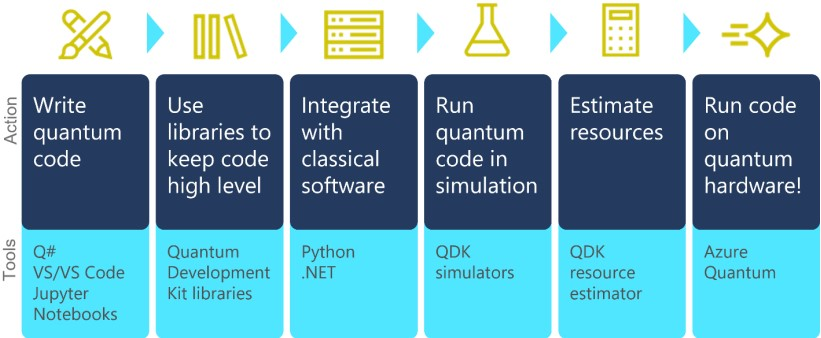
\includegraphics[width=3.5in]{QDK.jpg}
    \caption{Flujo de trabajo de ingeniería de software cuántico y herramientas QDK que respaldan cada paso.}
    \label{fig:quantum}
\end{figure}

Otro aspecto importante por mencionar es Quantum Katas, que son una serie de tutoriales y ejercicios diseñados para ayudar a las personas a entender la computación quántica, esta herramienta de igual forma fue creada por Microsoft con el fin de poder ayudar a los programadores a entender cómo funciona la computación cuántica. En este lenguaje se pretende explicar la sintaxis de Q\# (Q Sharp), estos ejercicios que proporciona Quantum Katas van desde nivel principiante hasta avanzado y cubre muchos temas relacionados con la computación cuántica (Mykhailova, 2020).

Después de hablar sobre muchos softwares creados en la computación cuántica hay que hacer una breve comparativa entre estos softwares, comparados con softwares de la actualidad, si observamos las características de la computación cuántica a nivel de software, en general podemos ver que son muy eficientes ya que realizan tareas en conjunto mediante la superposición y el entrelazamiento, estas características no las pueden utilizar en softwares convencionales, otra característica muy importante es que el nivel de velocidad que poseen estos softwares son descomunales, ya que como anteriormente se menciona en la criptografía, una desencriptación de una contraseña en un software convencional puede tardar 10 años, mientras que en un software cuántico es cuestión de segundos, esto hace que la eficiencia y la velocidad de este tipo de software sea de interés a nivel empresarial e industrial. 

Otro factor importante por considerar en la comparación de softwares cuánticos con softwares convencionales es la capacidad de procesamiento, ya que los ordenadores cuánticos pueden manejar grandes cantidades de datos y complejidad computacional de manera más eficiente que los ordenadores clásicos. Esto se debe a la capacidad de procesamiento simultáneo de múltiples estados cuánticos. De igual forma se pueden implementar nuevas aplicaciones debido a la capacidad de procesamiento y la precisión mejorada de los ordenadores cuánticos, ya que pueden permitir la creación de nuevos tipos de aplicaciones, como la simulación de procesos químicos y la optimización de redes neuronales. 

En conclusión, los softwares cuánticos ofrecen grandes capacidades en velocidades, capacidad y precisión, sin embargo, estos softwares se encuentran en desarrollo y existen muchos retos que deben ser superados, para poder llevar este software a un nivel de mejora más alto. A medida que los ordenadores y los algoritmos cuánticos sigan evolucionando, se espera que se abran nuevas posibilidades en áreas como la optimización, la simulación de sistemas complejos y la criptografía. 

\subsection{Aportes}
Hoy en día, no existe ningún campo o área en la cual la computación no tenga relevancia, desde trabajos profesionales hasta entretenimiento, la computación está presente en todo sitio, por otro lado, la computación cuántica tiene una visión de estar más enfocada al ámbito profesional, debido a sus abrumadoras capacidades, por lo tanto, se mencionarán algunas áreas en las cuales la computación cuántica podría desarrollar presencia en los próximos años:

\subsubsection{Procesamiento de imágenes} 
La computación cuántica presenta varias ventajas en este ámbito con respecto a la computación tradicional, varias de estas ventajas son: 
\begin{enumerate}
    \item Velocidad: las computadoras cuánticas tienen la capacidad de realizar operaciones en paralelo, lo cual acorta el tiempo de procesamiento drásticamente.

    \item Reducción de errores: este tipo de computación promete realizar cálculos más precisos, ya que analiza todos los casos posibles para dar con una respuesta.

    \item Reducción de recursos: al procesar imágenes de una forma más eficiente, es capaz de minimizar el consumo de otros recursos como lo es la memoria.
\end{enumerate}

En términos cotidianos, estos cambios no logran convencer a muchas personas, sin embargo, donde realmente se observan resultados sorprendentes es a la hora de procesar imágenes muy técnicas, por ejemplo, las imágenes médicas, donde imágenes en 3D pueden tener entre 512 y 1024 pixeles, en estos casos en concreto es donde se pueden observar cambios significantes, en especial en el tiempo requerido para procesar este tipo de imágenes. (Nouioua y Belbachir, 2023)

\subsubsection{Criptografía}
Actualmente no hay duda de que los avances en la tecnología y comunicaciones eléctricas han aumentado y son uno de los principales pilares de la tecnología en la edad moderna. En la actualidad se necesitan medios de seguridad confiables ya que muchas personas utilizan contraseñas poco seguras y esto provoca grandes vulnerabilidades a nivel de seguridad (Mavroeidis et al., 2018). 

A pesar de que la seguridad de la criptografía esté en juego, los algoritmos cuánticos pueden llegar a encriptar claves con un nivel de seguridad muy alto, ya que puede aumentar con el uso de espacios de clave más grandes. Además, se han introducido algoritmos que pueden romper los criptosistemas asimétricos actuales, cuya seguridad se basa en la dificultad de factorizar grandes números primos, ya que encontrar los factores primos de un número muy grande puede ser extremadamente difícil y lleva mucho tiempo para una computadora clásica. Por lo tanto, estos criptosistemas son considerados seguros porque sería muy difícil para un atacante obtener la clave privada necesaria para descifrar la información cifrada. 

\begin{itemize}
    \item{A}. Criptografía Simétrica

        En la criptografía simétrica, tanto el remisor como el emisor comparten una misma llave y un mismo sistema criptográfico, por el cual se encripta y descripta la información. Esta clave debe ser mantenida en secreto ya que es única, como la clave es la misma para ambos esto puede poner en riesgo la información, ya que con solo que una persona se entere de esta contraseña se hará pública. A causa de este problema se lanzó la criptografía asimétrica. 
    \item{B}. Criptografía asimétrica

        En la criptografía asimétrica, también llamada criptografía de clave pública (PKC), es una forma de encriptación donde las llaves o contraseñas vienen en parejas (Mavroeidis et al., 2018). 

        ¿A qué hace referencia esto? Se refiere a que se utilizan claves distintas para cifrar y descifrar, a diferencia de la simétrica, ahí se utiliza la misma clave para cifrado y descifrado, en la asimétrica se utiliza una clave privada y otra pública. La clave pública se comparte ampliamente y se utiliza para cifrar la información que se va a enviar a la persona que posee la clave privada. Solo el propietario de la clave privada correspondiente puede descifrar la información cifrada con la clave pública. La clave privada se mantiene en secreto y solo la persona que la posee puede usarla para descifrar la información cifrada con la clave pública. 
\end{itemize}

Un problema muy importante de la criptografía es el problema de factorización, ya que existe un algoritmo llamado criptosistema RSA, el cual se encarga de encriptar las contraseñas con algoritmos como los AES. Kirsch afirma que RSA es teóricamente vulnerable, ya que en un sistema cuántico donde se pueden realizar una cantidad de algoritmos eficientes que descriptan contraseñas, puede llegar a ser un problema para la seguridad de este tipo de datos y encriptaciones. 

Otro problema común es el problema del logaritmo discreto (DLP), en este se utilizan sistemas de seguridad como Diffie-Hellman y Elliptic Curve Cryptography para proteger la información. El DLP consiste en encontrar un número entero r que cumpla con cierta ecuación matemática. Resolver este problema es muy difícil y requiere de mucho tiempo y recursos computacionales. Debido a esto, los sistemas de seguridad son muy efectivos para proteger información. 

Por lo tanto, un sistema como una computadora cuántica puede llegar a resolver este tipo de problema en cuestión de segundos, entonces llegamos a la conclusión de que estos equipos pueden tanto dar mucha seguridad como vulnerabilidades en los sistemas criptográficos. 

En la actualidad la criptografía juega un rol importante en la seguridad de la tecnología, por ejemplo, los emails, contraseñas, transacciones bancarias, hasta sistemas de seguridad (Mavroeidis et al., 2018) 

Según NIST, las computadoras cuánticas van a acabar con los actuales esquemas de cifrado pública, ellos afirman el imparto de la computación cuántica en los esquemas criptográficos actuales (Mavroeidis et al., 2018). 

\begin{itemize}
    \item{A}. Algoritmo de Shor

        El algoritmo de Shor es un algoritmo que se utiliza para factorizar números enteros grandes en sus factores primos. Este algoritmo es muy importante en la criptografía asimétrica, ya que se utiliza en muchos sistemas como RSA, que tienen la dificultad de factorizar números enteros, a causa de esto este tipo de algoritmo se utiliza con el fin de facilitar este proceso y mejorar la seguridad. 

        El algoritmo de Shor utiliza la propiedad de la computación cuántica conocida como superposición y entrelazamiento para factorizar números enteros grandes de manera eficiente. La computación cuántica es capaz de realizar cálculos simultáneos utilizando qbits, que pueden estar en múltiples estados al mismo tiempo (Mavroeidis et al., 2018) 

        Este algoritmo funciona de la siguiente forma: Primero se utiliza la transformada de Fourier cuántica, que consiste en analizar señales periódicas, esto con el fin de encontrar el periodo de la función modular, la función modular se encarga de devolver el resto de la división de un número por otro. 

        En la segunda etapa del algoritmo, se utiliza el período encontrado en la primera etapa para calcular los factores primos del número entero. Esto se logra mediante el uso de una fórmula matemática que aprovecha la relación entre el período de la función modular y los factores primos del número entero. 
\end{itemize}

Después de haber mencionado que es la criptografía, como funciona, los tipos de algoritmos criptográficos que existen y sus funciones, un tema que es muy importante resaltar es la implementación de más seguridad en la criptografía en la actualidad, ya que como se conocen todos estos defectos y vulnerabilidades en estos sistemas, es importante implementar soluciones a estos problemas. 

Actualmente muchas empresas tales como NIST, anunciaron una convocatoria de propuestas de algoritmos en los cuales su idea es crear algoritmos resilientes a los ataques cuánticos, esto pasó en 2017. Luego en el 2018, Nist publicó los resultados de la primera ronda, que fueron un total de 82 algoritmos, de los cuales 59 cumplen con las características solicitadas (Mavroeidis et at., 2018). 

Todo esto es muy importante, ya que, si la criptografía cuántica avanza, nos garantizará una mejora en la seguridad de muchas plataformas tecnológicas, como las mencionadas anteriormente. Esto puede llegar a cambiar muchos aspectos cotidianos de las personas, por ejemplo, en el año 2023, se anunció una aplicación que guarda las contraseñas y las introduce como un código cifrado, esto es muy interesante ya que no se introduce una contraseña como tal, sino se introduce un pin el cuál se representa como la contraseña y es más difícil de descifrar. 

 \subsubsection{Finanzas} 
 En el ámbito de las finanzas y económica, se espera que se obtengan muchas ventajas, incluso que se llegue a transformar por completo este campo, todo gracias al exponencial crecimiento que podrían tener los algoritmos cuánticos.
 
Pese a que la computación está presente en las finanzas desde hace mucho tiempo, siguen existiendo problemas financieros, una gran cantidad de estos se podrían describir como deficiencias en la optimización, los cuales serían resueltos con el desarrollo de unidades más eficientes, sin embargo, existen otros problemas los cuales serían solucionados gracias a la computación cuántica, por ejemplo, en las ganancias. 

A la hora de hacer cualquier movimiento, se debe tener en cuenta el riesgo que este conlleva, es decir, se debe analizar si las ganancias serán mayores que las perdidas, a gran escala este análisis representa un enigma muy complejo, el cual puede ser resuelto con ayuda de las computadoras cuánticas, ya que estas tienen la capacidad de analizar una gran cantidad de casos posibles en cortos periodos de tiempo, entregando así los casos más beneficiosos. (Orús et al., 2019).

Por otro lado, se espera que con la ayuda de la computación cuántica se pueda tener una visión a futuro del mercado, es decir, que al evaluar un conjunto de casos puede determinar en que momento es mejor hacer movimientos y lograr predecir las tendencias que tendrá el mercado en un lapso. (Orús et al., 2019).

\subsubsection{Comunicación}
Una de las destrezas que se desean desarrollar en la computació cuántica es poder implementarla en la comunicación, específicamente en el internet, ya que este, pese a ser escencial en muchos aspectos de la actualidad, presenta algunas complicaciones como la seguridad y la velocidad. Por eso, se mencionarán algunos beneficios que traerá consigo el internet con el uso de computadoras cuánticas además de potenciales contratiempos que este podría presentar y el medio que servirá para este proceso.

El internet cuántico trae consigo ciertos avances importantes como un aumento significativo de la seguridad y la velocidad, gracias a los conceptos básicos de la cuántica como el entrelazamiento y la superposición, lo cual permite un transporte más rápido en comparación con los sistemas de comunicación de hoy en día. Como mencionan Caleffi et al. (2018), este proceso se llama Teleportación cuántica y se basa en la destrucción del qubit original que se reconstruye en el otro lado del canal, y así se cumple el teorema de no clonación. Para que esto suceda se envían 3 qubits, uno en cada extremo que estén en el mismo estado, y un tercero que va a medir la distancia, al cumplir el viaje el tercer quibit el que envía la información se destruye y vuelve a reconstruirse en el punto de llegada. 
\subsubsection{Medicina}
Además del procesamiento de imágenes, la computación cuántica puede significar un paradigma en la medicina, se espera que su mayor aporte sea para el tratamiento de cáncer, ya que, se presume que la computación cuántica será de gran utilidad en la radioterapia.

La radioterapia consiste en un procedimiento médico que se lleva a cabo en pacientes con cáncer, su objetivo es eliminar, mediante radiación, las células cancerígenas, sin embargo, se irradia una zona del cuerpo, no las células como tal, lo cual provoca que las células sanas también se vean comprometidas. 

La computación cuántica tiene la capacidad de realizar millones de cálculos en segundos, y es por eso que no le sería problema alguno encontrar las células cancerígenas, combinando estos tipos de tecnología, se podría crear un dispositivo para aplicar radioterapia que diriga la radiación específicamente a la posición en la que se encuentran las células que provocan el cancer (Gupta et al., 2023).

\subsection{Potenciales problemas de la computación cuántica}

La computación clásica a lo largo de su evolución ha presentado varios contratiempos en cuanto al transporte de la información, como lo son los cuellos de botella que son causados por memoria o hardware insuficientes, incluso algoritmos ineficientes. En cuanto a la computación cuántica, se puede hablar de cuellos de botella como la decoherencia de los procesos, esto ocurre en consecuencia de que las computadoras cuánticas, como se ha mencionado anteriormente, son muy sensibles a cualquier perturbación del medio, esto provoca que los qubits pierdan su principal caracteriztica que es su superposición, provocando así que funcionen como bits clásicos o incluso que dejen de funcionar. Si se da el caso de que funcionan como bits normales, los qubits acaban colapsando debido a que se les está pidiendo acciones que requieren múltiples cálculos, acciones que los qubits en estados de superposición podrían realizar sin problemas, pero al presentar esta afección, se crea un cuello botella ya que, se solicitan más cálculos de los  que se pueden realizar. (Zaidenberg et al. 2021).

Por otro lado, a pesar de que se han mencionado muchas ventajas que podría traer la computación cuántica, lo cierto es que también existen aspectos que amenazan con ser perjudicales, por ejemplo, en el ámbito de ciberseguridad y criptográfia, se teme que las computadoras cuánticas, al poder realizar cálculos extremadamente rápidos y precisos, puedan romper sistemas de cifrado en muy poco tiempo, cuando a las computadoras clásicas les tomaría años realizar estas acciones. (Bova et al., 2021). 

\newpage
\section{Conclusiones}
Como conclusión, si bien se puede demostrar que los computadores cuánticos poseen mayor potencia de procesamiento que los computadores tradicionales, pudiendo realizar cálculos que tomarían años, procesando imágenes mucho mejor que los computadores actuales o actuando en el área de la ciberseguridad. Estos aún no cumplen con todas las expectativas que se tienen sobre ellos, ya que presentan errores y complicaciones a la hora de trabajar. Además de que los computadores actuales tienen la ventaja de que son más amigables con la interacción usuario-máquina, ya que se han desarrollado para tener interfaces cómodas para las personas. Sin embargo, aún falta mucho por investigar sobre la computación cuántica, incluyendo maneras en que se pueda relacionar de manera cómoda con el usuario. Por lo que, si bien, hay mucha diferencia entre los computadores cuánticos y los tradicionales existe la posibilidad de que en el futuro se puedan desarrollar dispositivos híbridos que alcancen el balance entre ambas áreas.
Pese a todo lo anterior, se debe destacar que se debe tener sumo cuidado a la hora de crear dispositivos de esta magnitud, ya que al ser tan capaces, existe la posibilidad de que se pierda el control sobre estos, por lo tanto es importante que las investigaciones a futuro no se salgan de los conocimientos que se tienen sobre el tema, de esta forma, se pueden saber las consecuencias de lograr avances en la computación cuántica de una forma segura.



\clearpage
%----------

\subsection{Referencias}
Alexander, T. (2020). Qiskit pulse: programming quantum computers through the cloud with pulses. IOPSCIENCE. https://iopscience.iop.org/article/10.1088/2058-9565/aba404/meta

Awan, U., Hannola, L., Tandon, A., Goyal, R. K., y Dhir, A. (2022). Quantum computing challenges in the software industry. A fuzzy AHP-based approach. Information y Software Technology, 147, 106896. https://doi.org/10.1016/j.infsof.2022.106896

Ayoub, A., y Akram, J. (2021). Thermal entanglement of superconducting qubits for arbitrary interaction strength. Physica C: Superconductivity and its Applications, 591, 1353977. 10.1016/j.physc.2021.1353977.
https://doi.org/10.1016/j.physc.2021.1353977

Bova, F., Goldfarb, A., y Melko, R. G. (2021). Commercial applications of quantum computing. EPJ Quantum Technology, 8(1), 2. 10.1140/epjqt/s40507-021-00091-1 https://doi.org/10.1140/epjqt/s40507-021-00091-1 

Caleffi, M., Cacciapuoti, A., y Bianchi, G. (2018). Quantum internet. Paper presented at the 1-4. 10.1145/
3233188.
3233224 http://dl.acm.org/citation.cfm?id&#61;3233224

Gupta, S., Modgil, S., Bhatt, P. C., Chiappetta 
Jabbour, C. J., y Kamble, S. (2023). Quantum 
computing led innovation for achieving a more 
sustainable Covid-19 healthcare industry. 
Technovation, 120, 102544. 10.1016/j.technovation.2022.102544
https://doi.org/10.1016/j.technovation.2022.102544

Li, S., Wu, Y., & Chen, Y. (2023). A systematic and bibliometric review of the latest techniques in quantum-dot computers. Optik, , 170893. 10.1016/j.ijleo.2023.170893. https://doi.org/10.1016/j.ijleo.2023.170893

Liu, J., y Franklin, D. (2023). Introduction to quantum computing for everyone: Experience report. Paper presented at the SIGCSE 2023. Technica Symposium on Computer Science Education, 1 1157-1163. https://doi.org/10.1145/3545945.3569836 

Maier, C., Brydges, T., Jurcevic, P., Trautmann, N., Hempel, C., Lanyon, B. P., Hauke, P., Blatt, R., y Roos, C. F. (2019). Environment-assisted quantum transport in a 10-qubit network.American Physical Society (APS). 10.1103/physrevlett.122.050501 https://arxiv.org/pdf/1809.07680.pdf 

Mann, A., y Coolman, R. (2022). What is quantum mechanics? livescience.com. 
https://www.livescience.
com/33816-quantum-mechanics-explanation.html

Mavroeidis, V. (2018). The Impact of Quantum Computing on Present Cryptography. (IJACSA) International Journal of Advanced Computer Science and Applications, 9(3). 
1804.00200.pdf (arxiv.org)
https://doi.org/10.48550/arXiv.1804.00200

Metwalli, S. (2023). What Is Superposition? Built In. 
https://builtin.com/
software-engineering-perspectives
/superposition

Mykhailova, M. (2020). The Quantum Katas. Technical Symposium on Computer Science Education. https://doi.org/10.1145/3328778.3372543

Mykhailova, M. (2021). Testing Quantum Programs using Q and Microsoft Quantum Development Kit. Proceedings of the 2nd Quantum Software and Engineering Workshop. https://ceur-ws.org/Vol-3008/short6.pdf 

Nouioua, T., y Belbachir, A. H. (2023). The quantum computer for accelerating image processing and strengthening the security of information systems. Chinese Journal of Physics, 81, 104-124. 10.1016/j.cjph.2022
.11.006. 
https://doi.org/10.1016/j.cjph.2022.11.006

Orús, R., Mugel, S., y Lizaso, E. (2019). Quantum computing for finance: Overview and prospects. Reviews in Physics, 4, 100028. 10.1016/j.revip.2019.100028.
https://doi.org/10.1016/j.revip.2019.100028

S, N., Singh, H., y N, A. U. (2022). An extensive review on quantum computers. Advances in Engineering Software, 174, 103337. 10.1016/j.advengsoft.2022.103337.
https://doi.org/10.1016/j.advengsoft.2022.103337

Vadimov, A., Viitanen, T., Mörstedt, T., Ala-Nissila, T., y Möttönen, M. (2022). Single-junction quantum-circuit refrigerator. AIP Advances, 12(7), 075005. https://doi.org/10.1063/5.0096849

Xu, X., Wang, W., Sun, L., y Zou, C. (2022). Hybrid superconducting photonic-phononic chip for quantum information processing. Chip, 1(3), 100016. 10.1016/j.chip.2022.100016.
https://doi.org/10.1016/j.chip.2022.100016

Zaidenberg, D. A., Sebastianelli, A., Spiller, D., Le Saux, B., y Ullo, S. L. (2021).  Advantages and Bottlenecks of Quantum Machine Learning for Remote Sensing. Paper presented at the 5680-5683. 10.1109/IGARSS47720.2021.9553133 https://ieeexplore.ieee.org/document/9553133



\end{document}

